\documentclass[a4paper,11pt]{report}
\usepackage[]{amsmath}
\usepackage[]{physics} % \bra, \ket etc
\usepackage{graphicx} %Pour les figures je crois
\usepackage{hyperref}
\usepackage[
    backend=biber, 
    natbib=true,
    style=numeric-comp,
    sorting=none, %Pour faire apparaitre les refs dans l'ordre
    hyperref=true
]{biblatex} %Imports biblatex package
\addbibresource{Bib_ch1.bib} %Import the bibliography file

\usepackage{amssymb} %quelques symboles dont gtrsim /lesssim
\usepackage{subcaption} % package pour faire des subfigures
\usepackage{multirow} % package pour multirow/multicolumn
\usepackage{booktabs} % package pour top/mid/bottom rule
\usepackage{tcolorbox} % toujours plus de boites
\usepackage{xcolor} % Pour avoir des couleurs dans les équations

\title{}
\begin{document}
\chapter{Introduction to NV center and its common usage}
In this first chapter we will introduce the 

\section{The NV center as a physical object}
\subsection{Diamond overview}
\begin{figure}[h!]
\centering
\includegraphics[width=0.6\textwidth]{Figures/diamant_et_NV}
\caption{a) Drawing of a diamond with red fluorescent spots symbolizing NV centers. b) Zoom-in on the crystalline structure of an NV center}
\label{diamond+NV}
\end{figure}
We will start this chapter by discussing the physical aspect of the NV center, and of its host material, the diamond. We will cover some of the basic properties of diamond and of its most common defects before addressing the creation process of both diamonds and NV centers.

Fig. \ref{diamond+NV} illustrates a diamond with red fluorescent spots symbolizing NV centers, as well as the crystalline structure of the NV centers, where two carbon atoms are missing and one of them is replaced by a nitrogen atom.
\subsection{Diamond overview}
\begin{figure}[h!]
\centering
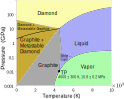
\includegraphics[width=0.6\textwidth]{Figures/phase_diagram_carbon_wiki}
\caption{Pressure-temperature phase diagram of elemental carbon. From wikipedia, adapted from \citep{bundy1989pressure, bundy1996pressure}.}
\label{carbon phase diagram}
\end{figure}

Diamond is a remarkable material in many aspects, it is famous for having the highest hardness and thermal conductivity of any natural material, and for its high optical refractive index and optical dispersion which makes it an extremely valuable crystal in jewelry.

Diamond is also famous for being extremely rare in nature, even though its only constituent, carbon, is one of the most abundant element on the Earth surface. The reason is that diamond is not the most stable phase of carbon under atmospheric pressure and temperature. This honor goes to the graphite which is found abundantly in coal. 

Fig. \ref{carbon phase diagram} shows the PT phase diagram of elemental carbon. We can see that diamond becomes the thermodynamically stable phase only for pressure above a few GPa, $10^4$ times higher than atmospheric pressure. Even though diamond is unstable under ambient conditions, the extremely high energy activation needed to break the sp$^3$ bond between two carbon atoms means that the kinematics of the $C_{\rm diamond} \to C_{\rm graphite}$ transition is almost completely frozen. In many ways diamonds are more stable than graphite under ambient condition due to their relative chemical inertness.

Where the thermodynamic equilibrium really matters is for the crystallization process. The higher pressure needed to reach the diamond-stable region can only be found naturally deep under the earth crust, typically between 150 and 240 km below sea level \citep{tappert2011diamonds}, which explain their rarity. It also explains why, despite many previous efforts, diamonds were synthetically produced for the first time only in 1953 \citep{barnard2000diamond}, more than 50 years after the first synthetic sapphires. To this day, artificial diamond synthesis remains an active field of research \citep{shenderova2019synthesis, achard2020chemical}.

Diamonds, either natural or artificial, are used in the lab and in industry for their extreme sturdiness, with applications ranging from abrasive to diamond anvil cells \citep{jayaraman1983diamond}. More recently, diamonds have been the object of optics and electronics applications. For both of these fields however, the focus is no longer solely on the diamond but also on the defects found inside it.

\subsection{Point defects in diamond}
\begin{figure}[h!]
\centering
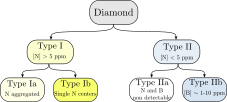
\includegraphics[width=0.9\textwidth]{Figures/Diamond_type}
\caption{Traditional classification of diamonds, based on \citep{tappert2011diamonds}}
\label{diamond type}
\end{figure}
Diamond in its intrinsic form is an insulator with a bandgap of of $\sim 5.47\ \rm eV$ and is transparent from far infrared to deep UV. As any crystal however, diamond is prone to defects. We will concentrate here on 0D point-like defects and omit structural defects such as dislocations, even though those too can affect the optical properties of the diamond \citep{collins2000colour}. 

Point-like defects can be constituted by the absence of a carbon atom (``vacancies"), an interstitial defect between two carbon atoms or the substitution of a carbon atom with another atom. These impurities result in unpaired electron or holes localized around the impurity site. This localization causes discrete energy levels for the holes or the electrons, some of which will lie inside the diamond bandgap and will impact the crystal optical and electrical properties. 

Defects with electronic transitions in the optical range are called ``colored centers" as they are responsible for the coloring of the gems.  H, He, Li, B, N,
O, Ne, P, Si, As, Ti, Cr, Ni, Co, Zn, Zr, Ag, W, Xe and Tl are known to form colored centers when introduced in diamond \citep{zaitsev2013optical, shenderova2019synthesis}, and each of these elements can form several defects. Nitrogen alone can form more than 50 different colored centers \citep{dobrinets2016hpht, ashfold2020nitrogen}.

Nitrogen, and to a lesser extant boron, are the most commonly found extrinsic elements in natural diamond. The traditional classification of diamond is presented in Fig. \ref{diamond type}. It is based on the N and B concentration, with a threshold of a few ppm (part per million) for each species as this was the smaller amount easily detectable through IR absorption. Type Ia diamonds contain clustered N defects such as the B-center which is the N$_4$V defect. In contrast, type Ib diamond mostly contains C-center which are single substitutional N$_s$ defects, also referred to as P1 centers in the spin community. Type IIb diamond contains B impurities which give them a blueish-grey color, and type IIa diamond contains no detectable impurities via IR absorption \citep{ashfold2020nitrogen}.

Nitrogen-vacancy centers are a rare occurrence in both natural diamonds and untreated synthetic diamonds, but we will see later that the much more common N$_s$ defects can be converted in NV centers. When working with NV centers, the starting crystal is therefore often a type Ib if one wants to work with ensemble, or a type IIa if one wants to work with single NV centers.

The boron defects are mainly studied in the context of p-doped diamond semi-conductor: a concentration of [B] $\approx 1000\ \rm ppm$ is needed to achieve a significant overlap between the impurity sites, which turns the diamond into a semi-metal \citep{macpherson2015practical}.Other defects of interest, generally not present naturally but introduced voluntarily, include P and S defects to create n-doped diamond \citep{das2022diamond} (still an active field of research), as well as group IV-vacancy defects (SiV, GeV, SnV, PbV) for quantum optics application \citep{bradac2019quantum}. 

The NV center however remains by far the most studied defect in diamond due to its unique spin properties which will be explained below.

\subsection{Creation of synthetic diamond for NV application}







\printbibliography
\end{document}
